\documentclass{report}
\newcommand*{\twodot}{\mathrel{\rlap{%
			\raisebox{0.3ex}{$\cdot$}}%
		\raisebox{-0.3ex}{$\cdot$}}%
}
\usepackage{tikz}
\usepackage{amsmath}
\tikzstyle{vertex}=[circle,draw,inner sep=0pt,minimum size=0pt]
\newcommand{\vertex}{\node[vertex]}

\usepackage{arxiv}
\usepackage{makecell}

\usepackage[utf8]{inputenc} % allow utf-8 input
\usepackage[T1]{fontenc}    % use 8-bit T1 fonts
\usepackage{hyperref}       % hyperlinks
\usepackage{url}            % simple URL typesetting
\usepackage{booktabs}       % professional-quality tables
\usepackage{amsfonts}       % blackboard math symbols
\usepackage{nicefrac}       % compact symbols for 1/2, etc.
\usepackage{microtype}      % microtypography
\usepackage{lipsum}		% Can be removed after putting your text content
\usepackage{graphicx}



\title{a low rank convolution operation generating numerous feature maps}

%\date{September 9, 1985}	% Here you can change the date presented in the paper title
%\date{} 					% Or removing it

\author{ \href{https://orcid.org/0000-0000-0000-0000}{
\includegraphics[scale=0.06]{orcid.png}\hspace{1mm}Reza Mohajernoei}\\
	Department of Computer Science\\
	Tarbiat Modares University\\
	\texttt{m.reza@modares.ac.ir} \\
	%% examples of more authors
	\And
	\href{https://orcid.org/0000-0000-0000-0000}{
\includegraphics[scale=0.06]{orcid.png}\hspace{1mm}Mansoor Rezghi}\thanks{https://www.modares.ac.ir/~rezghi}  \\
	Department of Computer Science\\
	Tarbiat Modares University\\
	\texttt{rezghi@modares.ac.ir} \\
	%% \AND
	%% Coauthor \\
	%% Affiliation \\
	%% Address \\
	%% \texttt{email} \\
	%% \And
	%% Coauthor \\
	%% Affiliation \\
	%% Address \\
	%% \texttt{email} \\
	%% \And
	%% Coauthor \\
	%% Affiliation \\
	%% Address \\
	%% \texttt{email} \\
}

% Uncomment to remove the date
%\date{}

% Uncomment to override  the `A preprint' in the header
%\renewcommand{\headeright}{Technical Report}
%\renewcommand{\undertitle}{Technical Report}

%%% Add PDF metadata to help others organize their library
%%% Once the PDF is generated, you can check the metadata with
%%% $ pdfinfo template.pdf
\hypersetup{
pdftitle={A template for the arxiv style},
pdfsubject={q-bio.NC, q-bio.QM},
pdfauthor={David S.~Hippocampus, Elias D.~Striatum},
pdfkeywords={First keyword, Second keyword, More},
}

\begin{document}
\maketitle

\begin{abstract}
	

	Convolutional Neural Network is an essential tool in machine learning used in many applications and computers on various scales. For instance, one can see their role in different applications such as Machine Vision, Natural Language Processing, and financial data. Recently, Convolutional Neural Networks have shown satisfying and even fantastic performance in different applications. This ability of Neural Networks sometimes surpasses human categorization or recognition. Despite their advantages, Neural Networks involve some challenges as well. Numerous parameters consumption requires powerful calculation tools to solve the problems. Some solutions have been provided to overcome this issue. Different methods exist to improve Convolutional Neural networks. One of these approaches is based on tensor decompositional methods. Because The parameters (Kernel-Filter) between two layers of Convolutional Neural Network is always a four-dimensional tensor. In tensor methods, the parameter numbers are usually sought to be reduced using tensor decompositions. Therefore different approximations of convolution operations could be found by these methods. Hence, the concept of tensor, as a critical solution, got into Neural Networks literature.
	It should be noted that although recently have been tensor appearing in a lot of articles and research, Neural Networks had been based on a specialized condition of tensor application because tensors were a generalization of weights vectors and in-layer connections matrices. Consequently, tensors have shown a significant usage to replace the lower dimensions, representations of the layer-wise connections approach towards utilizing this concept have been extending. In this research, we tend to announce a mechanism inspired by some studies in this field and combining them with algebraic concepts to improve the Convolutional Neural Networks, which consume fewer resources with more negligible effect on the accuracy, and in the end, the experimental results will be reported.
	

\end{abstract}


% keywords can be removed
\keywords{ Deep Neural Networks
	\and
	 Tensor product
	\and
	 Contractive dot
	\and
	 Convolutional operation
	\and
	 Convolutional Neural Networks}


\section{Introduction}

\paragraph*{}
Convolutional Neural Networks have shown their advantages over the other methods in the last decade. Initially announced before the millennium
\cite{hinton}
and evolved during the recent years, Convolutional Neural Network has a wide range of applications such as computer vision
\cite{vis2,vis1,vis3}
, natural language processing
\cite{nlp2,nlp1}
, and biomedical
\cite{bio1,bio2}
or financial analysis
\cite{fin2,fin1}
. Despite their prominent  ubiquity, Convolutional Networks suffer from several difficulties, such as the need for the mass amount of data to be appropriately trained, numerous parameters to build a network which is also called memory complexity; learning these parameters in every deep learning solution is a complex optimization task
\cite{danish}
%Deep learning applications and challenges in
%big data analytics
%Maryam M Najafabadi1, Flavio Villanustre2, Taghi M Khoshgoftaar1, Naeem Seliya1,
%Randall Wald1* and Edin Muharemagic
. Hence, the convolutional neural network is a time-consuming solution, also. A higher number of parameters expands the search space, and consequently, the accuracy grows. In line with more advanced hardware and new generations of processing units
\cite{gpu}
, the network designers and researchers announced new architectures in which millions of parameters were utilized to extract better results with current facilities
\cite{mobilenets,alexnet,resnets,vgg}
. Although this equipment paved the way for many high-quality and precise results in different fields, advances, in turn, caused inattention to the essence of thriftiness about the resource.

\paragraph*{}
 Although they are known as a real solution for most of the machine learning tasks, and they are still under development, the curse of resource consumption has remained an issue. Besides introducing novel architectures requiring less floating-point operations and memory, many research pieces have focused on hashing technique
\cite{hashteq}
, pruning 
\cite{prun}
and fine-tuning
\cite{fine}
CNN. However, few have tried changing the traditional convolution operation mechanism, which affects the overall memory and computation cost by itself
\cite{convop1,
	convop2,
	convop3,
	convop4,convop5}. Across a CNN, from input towards output, we encounter tensors with different dimensions and sizes
\cite{tenmatvec}
. Hence, multilinear operations suggest solutions to overcome this challenge and have turned into a fundamental remedy for such a problem
\cite{convop1,trl}
.
In this work, while applying a multilinear method instead of the old-fashioned convolution with less resource usage, we generate even more feature maps for the network's successive layers. Theoretical and experimental results show that the new operation outperforms the traditional ones in parameter consumption and computation complexity.


\paragraph*{}
Techniques such as pruning and fine-tuning the networks have turned out to be helpful but still redundant\cite{redundancy}. One of the trickiest ways to reduce both the time and memory complexity of a network is to change the convolution's essential core functions. Some works suggested changing the mechanism of convolution, whether by changing the filter\cite{convop1,
	convop2,
	convop3,
	convop4,convop5,danish} or even the order and stages of convolution in a layer\cite{depthwise,mobilenets}. Some tried to change the way fully connected perform using linear algebraic decompositions\cite{trl}.

\paragraph*{}
In this paper, we will not propose an architecture involving multiple convolutions one after another\cite{resnets,alexnet,mobilenets,vgg}, nor are we going to break the convolution into several stages\cite{depthwise}. Instead, we get major inspiration from changing the core functionality of convolution thanks to tensorial and linear algebraic concepts\cite{convop1}. We will at first discuss similar ideas on designing novel convolutions, those which have shown their advantages in practice. Then the experiments demonstrate why this method is a suitable alternative for the standard convolution. Finally, a conclusion will sum the discussion in a nutshell.

\section{Related Work}
\paragraph*{}
Besides a means of better illustrating the competence of Deep Neural Networks
\cite{anim4}
Tensor methods have been used in different machine learning applications, such as learning latent variable models
\cite{anim1} and developing recommender systems
\cite{anim10},
Several research applied tensor learning
\cite{anim17}
and tensor decomposition
\cite{anim9,anim15} to Deep Neural Networks. Furthermore, they have been used in multi-task learning 
\cite{anim20}, and sharing residual
units
\cite{anim3} as well.


\paragraph*{}
Recently, Convolutional neural networks have drawn the spotlight on themselves though they use a high amount of unnecessary memory and calculations
\cite{trl}. In some architectural solutions, such as Resnets
\cite{resnets}, changing the order of convolutional layers along a network has been a method to increase the accuracy of the convolutional neural networks in different applications. The expense of memory and time has led researchers to design well-known cost-efficient networks
\cite{resnets,mobilenets,alexnet,vgg}. The efficiency results from different aspects. Some efforts have shown their advantages successfully, such as TRL networks which concentrated on the final layers, made use of tensor decompositions to lessen the cost of convolutional neural networks\cite{trl}. Another outstanding idea helping to improve Convolutional Neural Networks is the bottleneck layer deployed by ResNets architecture which has been undeniably successful in image classification, and object detection\cite{resnets}. Another critical example is MobileNets comprising several layers in each of which separates the convolution operation into two stages\cite{mobilenets}  such that At the first stage, depthwise convolution is applied on the input, then its output is fed to the second stage performing one by one convolution which is called pointwise
\cite{depthwise}. This idea has turned out to be reasonable in both performances and resource consumption\cite{mobilenets}. Considering the research on improving Neural Networks in terms of the core convolution function\cite{convop1}, it is evident that most researchers have spent significant effort and time manipulating the existing structures and known architectures, modifying the order of layer placements, normalizations, pooling layers, and even activation functions. With the rise of AlexNets, Convolutional Neural network has been revolutionized; the excellence of Graphical Processing Units has neutralized even the dramatic increase in the number of parameters
\cite{gpu}
. On the other hand, only recently has potential linear algebra power shown its role in reordering the convolution operation
\cite{danish,convop1,trl}.
An exquisite idea to reduce the cost of a Convolutional Neural Network is a low-rank approximation of the convolution operation.
\cite{convop1}
A good example of low rank approximation can be shown by the formula that follows:



\begin{equation*}
\tilde{W}^{c}_{n} \simeq \sum ^{K}_{k=1} V^{c} _{k}(H^{k}_{n})^{T}
\end{equation*}


In this formula, subscripts and superscripts stand for the channel index and the corresponding kernel and $K$ is the hyper parameter which works as a rank controller of the approximation matrix. Here,   $\tilde{W}^{c}_{n} $ just represents a two-dimensional kernel of the $n$th filter that applies on $c$th channel. Also, 
$ V^{c} _{i}\in R^{R\times w_1\times 1\times C}$ 
and
$ H^{i}_{n}\in R^{N\times 1\times w_2\times R} $.
With this filter and applied on the input $X$, convolution operation applies as follows:



\begin{equation*}
\tilde{W}_{n}* X = \sum^{C}_{c=1}\sum^{R}_{i=1}H_{n}^{i}(V_{i}^{c})^T*X^c = \sum^{R}_{i=1}H_{n}^{i} *\bigg( \sum^{C}_{c=1}V_{i}^{c}*X^c\bigg)
\end{equation*}

in which 
$X\in R^{X\times Y\times C}  $
and
$\tilde{W}_{n}\in R^{w_1\times w_2\times C}$
.

\paragraph*{}
This method aims at convolving with two types of parameter sharing. First is sharing all right singular vectors $ H^{k}_{n} $ along all the input channels $C$ and in the $n$th filter, while the second ensures parameter sharing via left singular vectors $ V^{c} _{k} $ along all of the $N$ filters
\cite{convop1}
.










\section{
	Proposed Method
}
\paragraph*{}
Before getting over the main description of the main idea of the proposed method, we need to introduce some notations using which we will describe the method.

subsection{
	prerequisites
}



\subsubsection{
	Rank-1 tensor
	\cite{kolda}
}

\paragraph*{}
An N-way tensor $ X \in R^{I_1\times I_2\times \dots \times I_N} $ is rank one if it
can be written as the outer product of $ N $ vectors, i.e.,



\begin{equation*}
X = a^{(1)} \bullet a^{(2)} \bullet \dots \bullet a^{(N)}.
\end{equation*} 

The symbol $"\bullet"$ represents the vector outer product. This means that each element
of the tensor is the product of the corresponding vector elements:


\begin{equation*}
x_{i_{1}i_{2}\dots i_{N}} = a^{(1)}
_{i_{1}} a^{(2)}
_{i_{2}} \dots a^{(N)}
_{i_{N}}\;\;
\;for \;\; all \;\;\;\;\; 1 \le i_n \le I_{n}.
\end{equation*} 



\begin{figure}[h!]
	\begin{center}
		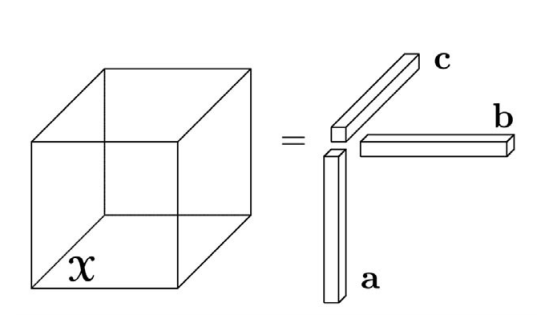
\includegraphics[height=5cm]{rankone.png}
	\end{center}
	\label{rankone}
	\caption{$Rank-one\; third-order\; tensor, X = a \bullet b \bullet c.\; The (i, j, k)\; element\; of\; X \;is \;given \;by \;x_{ijk}\; =\;
		a_ib_jc_k.$}
\end{figure}


Figure
\ref{rankone}
illustrates $X = a \bullet b \bullet c$, a third-order rank-one tensor.





\begin{figure}[h!]
	\begin{center}
		\label{fi2}
		
		
		\resizebox{0.7 \textwidth}{!}{%
			
			
			\begin{tikzpicture}
		% % % % % % % % % % % % % % % % % % % % % % % % % % % % % 
		
		
		
		\vertex  [label={\LARGE \vdots}] (x2) at (-6.25,-0.3) [] {};
		
		\vertex  [label={\LARGE +}] (x1) at (-3.25,0.7) [] {};
		\vertex  [label={\LARGE \vdots}] (x2) at (-3.25,-0.3) [] {};
		\vertex  [label={\LARGE +}] (x3) at (-3.25,-1.3) [] {};
		\vertex  [label={\LARGE Inputs}] (x3) at (-8,5) [] {};
		\vertex  [label={\LARGE The stack of kernels}] (x4) at (-3.25,5.1) [] {};
		\vertex  [label={\LARGE Output channel }] (x5) at (4,5.1) [] {};
		% % % % % % % % % % % % % % % % % % % % % % % % % % % % %  
		%*********************
		\vertex  [] (a1) at (-10,-4) [] {};
		\vertex  [] (a2) at (-10,4) [] {};
		\vertex  [] (a3) at (-6,4) [] {};
		\vertex  [] (a4) at (-6,-4) [] {};
		%********************
		\vertex  [] (b1) at (-9,-3.5) [] {};
		\vertex  [] (b2) at (-9,-1.5) [] {};
		\vertex  [] (b3) at (-7,-1.5) [] {};
		\vertex  [] (b4) at (-7,-3.5) [] {};
		\vertex  [label={\Large $x(\twodot,\twodot,N)$}] (b5) at (-8,-2.9) [] {};
		%***********************
		\vertex  [] (c1) at (-9,3.5) [] {};
		\vertex  [] (c2) at (-9,1.5) [] {};
		\vertex  [] (c3) at (-7,1.5) [] {};
		\vertex  [] (c4) at (-7,3.5) [] {};
		\vertex  [label={\Large $x(\twodot,\twodot,1)$}] (c5) at (-8,2.1) [] {};
		%***********************
		\vertex  [label={\LARGE *\;\;\;}] (k1) at (-4.5,2) [] {};
		\vertex  [label={\LARGE *\;\;\;}] (k2) at (-4.5,-3) [] {};
		\vertex  [label={\LARGE $W(\twodot,\twodot,1,j)$}] (k3) at (-2.8,2.1) [] {};
		\vertex  [label={\LARGE $W(\twodot,\twodot,N,j)$}] (k4) at (-2.8,-2.9) [] {};
		%***********************
		\vertex  [] (d1) at (-0.8,-2.6) [] {};
		\vertex  [] (d2) at (0.2,-2.6) [] {};
		\vertex  [] (d3) at (0.2,0) [] {};
		\vertex  [] (d4) at (1.2,0) [] {};
		\vertex  [] (d5) at (1,-0.2) [] {};
		\vertex  [] (d6) at (1,0.2) [] {};
		%*******************
		\vertex  [] (f1) at (2,-4) [] {};
		\vertex  [] (f2) at (2,4) [] {};
		\vertex  [] (f3) at (6,4) [] {};
		\vertex  [] (f4) at (6,-4) [] {};
		%***********************
		\vertex  [] (e1) at (3,-1) [] {};
		\vertex  [] (e2) at (3,1) [] {};
		\vertex  [] (e3) at (5,1) [] {};
		\vertex  [] (e4) at (5,-1) [] {};
		\vertex  [label={\Large $y(\twodot,\twodot,j)$}] (e5) at (4,-0.4) [] {};
		%***************
		
		\path
		% % % % % % % % % % % % % % % % %
		%**************
		(a1) edge [] (a2)
		(a1) edge [] (a4)
		(a2) edge [] (a3)
		(a3) edge [] (a4)
		%**************
		(b1) edge [] (b2)
		(b1) edge [] (b4)
		(b2) edge [] (b3)
		(b3) edge [] (b4)
		%********************
		(c1) edge [] (c2)
		(c1) edge [] (c4)
		(c2) edge [] (c3)
		(c3) edge [] (c4)
		%********************
		(d1) edge [] (d2)
		(d2) edge [] (d3)
		(d3) edge [] (d4)
		(d4) edge [] (d5)
		(d4) edge [] (d6)
		%**************
		(f1) edge [] (f2)
		(f1) edge [] (f4)
		(f2) edge [] (f3)
		(f3) edge [] (f4)
		%**************
		(e1) edge [] (e2)
		(e1) edge [] (e4)
		(e2) edge [] (e3)
		(e3) edge [] (e4)
		%********************
		;			\end{tikzpicture}}
	\caption{
	ُThe $j$th channel is generated by summation of product of two tensors in the manner shown above in a standard convolution operation}
\end{center}
\end{figure}


\subsubsection{
	Fibers
	\cite{kolda}
}

\paragraph*{}
Fibers are the higher-order analogue of matrix rows and columns. A fiber is
defined by fixing every index but one. A matrix column is a mode-1 fiber and a
matrix row is a mode-2 fiber. Third-order tensors have the column, row, and tube fibers,
denoted by $ x_{:jk} $, $ x_{i:k} $, and $ x_{ij:} $, respectively; see 
\ref{fibers}
When extracted from the
tensor, fibers are always assumed to be oriented as column vectors.






\subsubsection{
	Tensor-matrix multiplication\cite{rezghi}
}

\paragraph*{}
Let us assume $ X \in R^{J\times K\times L} $ and $ W\in R^{M\times J} $.
The Tensor-matrix multiplication is defined as follows:


\begin{equation*}
y_{mkl} = \sum^J_{j=1}W_{mj}x{jkl}.
\end{equation*} 

Where $Y \in R^{M\times K\times L}$This means that all column vectors (mode-1 fibers) in the order-3 tensor are multiplied by the matrix
W . Similarly, mode-2 multiplication by a matrix X means that all row vectors (mode-2 fibers) are
multiplied by the matrix X. Mode-3 multiplication is analogous.
In the case when tensor-matrix multiplication is performed in all modes in the same formula, we
omit the subscripts and write:


\begin{equation*}
(A,B,C)\bullet{X}
\end{equation*} 

Where the mode of each multiplication is understood from the order in which the matrices are given.






\subsection{Thrifty output feature map generator as a Convolutional Layer}

\paragraph*{}
We can develop tensor methods to reduce the problem size being inspired by previous papers\cite{danish,mobilenets}. We can present a new generator formula like:

\begin{figure}[h!]
	\begin{center}
		\label{fi2}
		
		
		\resizebox{0.7 \textwidth}{!}{%
			
			
			\begin{tikzpicture}
			% % % % % % % % % % % % % % % % % % % % % % % % % % % % % 
			\vertex  [label={\LARGE \vdots}] (x1) at (-9,-1.8) [] {};
			\vertex  [label={\LARGE \vdots}] (x2) at (-3.25,-1.8) [] {};
			\vertex  [label={\LARGE Inputs}] (x3) at (-9,3) [] {};
			\vertex  [label={\LARGE Inputs,Kernels}] (x4) at (-3.25,3.1) [] {};
			\vertex  [label={\LARGE A sample output}] (x5) at (3,3.1) [] {};
			\vertex  [] (j1) at (-10,-1) [] {};
			\vertex  [] (j2) at (-10,1) [] {};
			\vertex  [] (j3) at (-8,1) [] {};
			\vertex  [] (j4) at (-8,-1) [] {};
			\vertex  [] (j5) at (-9.5,-0.5) [] {};
			\vertex  [] (j6) at (-9.5,0.5) [] {};
			\vertex  [] (j7) at (-8.5,0.5) [] {};
			\vertex  [] (j8) at (-8.5,-0.5) [] {};
			\vertex  [] (j9) at (-9,0) [] {};
			\vertex  [label={$(i,j)$}] (j10) at (-9,2) [] {};
			\vertex  [] (j11) at (-9.2,1.8) [] {};
			\vertex  [] (j12) at (-8.8,1.8) [] {};
			\vertex  [] (j13) at (-8.5,-0.1) [] {};
			\vertex  [] (j14) at (-8.5,0.1) [] {};
			\vertex  [] (j15) at (-7,-0.1) [] {};
			\vertex  [] (j16) at (-7,0.1) [] {};
			\vertex  [] (j17) at (-6.8,0) [] {};
			\vertex  [] (j18) at (-7.3,-0.25) [] {};
			\vertex  [] (j19) at (-7.3,0.25) [] {};
			%*********************
			\vertex  [] (b1) at (-4.5,-0.7) [] {};
			\vertex  [] (b2) at (-4.5,0.7) [] {};
			\vertex  [] (b3) at (-5,0) [] {};
			\vertex  [] (b5) at (-4.5,-0.5) [] {};
			\vertex  [] (b6) at (-4.5,0.5) [] {};
			\vertex  [] (b7) at (-3.5,0.5) [] {};
			\vertex  [] (b8) at (-3.5,-0.5) [] {};
			\vertex  [label={\LARGE $,$}] (b9) at (-3.25,-0.25) [] {};
			\vertex  [label=below:{$+$}] (p1) at (-3.25,-0.75) [] {};
			\vertex  [] (b10) at (-3,-0.5) [] {};
			\vertex  [] (b11) at (-3,0.5) [] {};
			\vertex  [] (b12) at (-2,0.5) [] {};
			\vertex  [] (b13) at (-2,-0.5) [] {};
			\vertex  [] (b14) at (-2,-0.7) [] {};
			\vertex  [label={$W(\twodot,\twodot,1)$}] (b15) at (-2,0.7) [] {};
			\vertex  [] (b16) at (-1.5,0) [] {};
			% % % % % % % % % % % % % % % % % % % % % % % % % % % % %  
			%*********************
			\vertex  [] (a1) at (-10,-4) [] {};
			\vertex  [] (a2) at (-10,-2) [] {};
			\vertex  [] (a3) at (-8,-2) [] {};
			\vertex  [] (a4) at (-8,-4) [] {};
			\vertex  [] (a5) at (-9.5,-3.5) [] {};
			\vertex  [] (a6) at (-9.5,-2.5) [] {};
			\vertex  [] (a7) at (-8.5,-2.5) [] {};
			\vertex  [] (a8) at (-8.5,-3.5) [] {};
			\vertex  [] (a13) at (-8.5,-3.1) [] {};
			\vertex  [] (a14) at (-8.5,-2.9) [] {};
			\vertex  [] (a15) at (-7,-3.1) [] {};
			\vertex  [] (a16) at (-7,-2.9) [] {};
			\vertex  [] (a17) at (-6.8,-3) [] {};
			\vertex  [] (a18) at (-7.3,-3.25) [] {};
			\vertex  [] (a19) at (-7.3,-2.75) [] {};
			%********************
			\vertex  [] (c1) at (-4.5,-3.7) [] {};
			\vertex  [] (c2) at (-4.5,-2.3) [] {};
			\vertex  [] (c3) at (-5,-3) [] {};
			\vertex  [] (c5) at (-4.5,-3.5) [] {};
			\vertex  [] (c6) at (-4.5,-2.5) [] {};
			\vertex  [] (c7) at (-3.5,-2.5) [] {};
			\vertex  [] (c8) at (-3.5,-3.5) [] {};
			\vertex  [label={\LARGE $,$}] (c) at (-3.25,-3.25) [] {};
			\vertex  [label={$+$}] (p2) at (-3.25,-2.25) [] {};
			\vertex  [] (c10) at (-3,-3.5) [] {};
			\vertex  [] (c11) at (-3,-2.5) [] {};
			\vertex  [] (c12) at (-2,-2.5) [] {};
			\vertex  [] (c13) at (-2,-3.5) [] {};
			\vertex  [] (c14) at (-2,-3.7) [] {};
			\vertex  [label={$W(\twodot,\twodot,N)$}] (c15) at (-2,-2.3) [] {};
			\vertex  [] (c16) at (-1.5,-3) [] {};
			
			%*********************
			\vertex  [] (f1) at (2,-2.5) [] {};
			\vertex  [] (f2) at (2,-0.5) [] {};
			\vertex  [] (f3) at (4,-0.5) [] {};
			\vertex  [] (f4) at (4,-2.5) [] {};
			\vertex  [] (f5) at (2.5,-2) [] {};
			\vertex  [] (f6) at (2.5,-1) [] {};
			\vertex  [] (f7) at (3.5,-1) [] {};
			\vertex  [] (f8) at (3.5,-2) [] {};
			\vertex  [] (f9) at (3,-1.5) [] {};
			\vertex  [label=below:{$y^{ij}$}] (f10) at (3,-3.5) [] {};
			\vertex  [] (f11) at (3.2,-3.3) [] {};
			\vertex  [] (f12) at (2.8,-3.3) [] {};
			% % % % % % % % % % % % % % % % %
			\vertex  [] (d1) at (-0.8,-3) [] {};
			\vertex  [] (d2) at (0.2,-3) [] {};
			\vertex  [] (d3) at (0.2,-1.5) [] {};
			\vertex  [] (d4) at (1.2,-1.5) [] {};
			\vertex  [] (d5) at (1,-1.3) [] {};
			\vertex  [] (d6) at (1,-1.7) [] {};
			\path
			% % % % % % % % % % % % % % % % %
			(j1) edge [] (j2)
			(j1) edge [] (j4)
			(j2) edge [] (j3)
			(j3) edge [] (j4)
			(j5) edge [] (j6)
			(j5) edge [] (j8)
			(j6) edge [] (j7)
			(j7) edge [] (j8)
			(j9) edge [] (j10)
			(j10) edge [] (j11)
			(j10) edge [] (j12)
			(j13) edge [] (j15)
			(j14) edge [] (j16)
			(j17) edge [] (j18)
			(j17) edge [] (j19)
			%**************
			(b1) edge [] (b3)
			(b2) edge [] (b3)
			(b5) edge [] (b6)
			(b5) edge [] (b8)
			(b6) edge [] (b7)
			(b7) edge [] (b8)
			(b10) edge [] (b11)
			(b10) edge [] (b13)
			(b11) edge [] (b12)
			(b12) edge [] (b13)
			(b16) edge [] (b14)
			(b16) edge [] (b15)
			%**************
			(a1) edge [] (a2)
			(a1) edge [] (a4)
			(a2) edge [] (a3)
			(a3) edge [] (a4)
			(a5) edge [] (a6)
			(a5) edge [] (a8)
			(a6) edge [] (a7)
			(a7) edge [] (a8)
			(a13) edge [] (a15)
			(a14) edge [] (a16)
			(a17) edge [] (a18)
			(a17) edge [] (a19)
			%********************
			(c1) edge [] (c3)
			(c2) edge [] (c3)
			(c5) edge [] (c6)
			(c5) edge [] (c8)
			(c6) edge [] (c7)
			(c7) edge [] (c8)
			(c10) edge [] (c11)
			(c10) edge [] (c13)
			(c11) edge [] (c12)
			(c12) edge [] (c13)
			(c16) edge [] (c14)
			(c16) edge [] (c15)
			% % % % % % % % % % % % % % % % %
			(f1) edge [] (f2)
			(f1) edge [] (f4)
			(f2) edge [] (f3)
			(f3) edge [] (f4)
			(f5) edge [] (f6)
			(f5) edge [] (f8)
			(f6) edge [] (f7)
			(f7) edge [] (f8)
			(f9) edge [] (f10)
			(f10) edge [] (f11)
			(f10) edge [] (f12)
			%*************
			(d1) edge [] (d2)
			(d2) edge [] (d3)
			(d3) edge [] (d4)
			(d4) edge [] (d5)
			(d4) edge [] (d6)
			;
			\end{tikzpicture}}
		\caption{
			The final matrice is output by reshaping the resulting vector}
	\end{center}
\end{figure}

\begin{equation*}
Y(:,:,j) = \sum^N_{l=1} W(:,:,l,j) \ast X(:,:,l)
\end{equation*} 

where the bias addition expression has been omitted for simplicity and $ * $
represents the convolution operation and has been defined, before. To simplify the formula, we eliminate the index 
$ j $
from it:

\begin{equation*}
Y = \sum^N_{l=1} W(:,:,l) \ast X(:,:,l)
\end{equation*} 

In other words, as in figure
\ref{fi2}
 the 
$ (i,j) $th element of the output matrice $ Y $
obtains by the formula:

\begin{equation} \label{eq:v}
y^{i,j} = \sum^N_{l=1}\big\langle X^{i,j}_{l},W(:,:,l)\big\rangle
\end{equation} 

\iffalse



\begin{figure}[h!]
	\begin{center}
		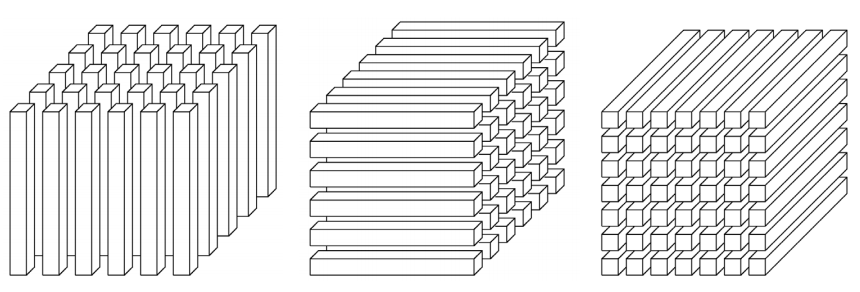
\includegraphics[height=5cm]{fibers.png}
	\end{center}
	\label{fibers}
	\caption{
		Fibers of a 3rd-order tensor. from left, respectively:
		$ Mode-1 \; (column)fibers,\; Mode-2 \; (row)\; fibers \;and  \; Mode-3 \; (tube) \;  fibers$}
\end{figure}

\fi




In which, the spacial size of
$ X^{i,j}_{l} $th patch is equal to the $ l $ th channel of the filter.
Supposing 
$x^{i,j}\in R^{W_{1}\times W_{2}\times N}$
and
$ x^{i,j}(:,:,l)= X^{i,j}_{l} $
،
then :

\begin{equation} \label{eq:544}
y^{i,j} = \sum^N_{l=1}\big\langle X^{i,j}_{l},W(:,:,l)\big\rangle = \big\langle x^{i,j},W\big\rangle
\end{equation} 

In which:
$ \big\langle , \big\rangle $
Represents inner product of two tensors. In 
\cite{danish},
assuming 
$ W = a\bullet b \bullet c  $
Means outer product of 3 vectors and therefore:

\begin{equation} \label{eq:545}
y^{i,j} =  \big\langle x^{i,j},a \bullet b \bullet c \big\rangle
\end{equation} 

Based on the inner and matrix product property between a tensor and a matrix(vector,)
\cite{rezghi}:

\begin{equation} \label{eq:546}
y^{i,j} = (a,b,c)_{1:3}\cdot x^{i,j}
\end{equation} 

In fact,
\cite{danish}
Assumes that tensor shaped filter

$ W \in R^{W_{1}\times W_{2}\times N} $
is of rank 1. Generally if we have supposed
$W = \sum^{R}_{r=1}a_{r}\bullet b_{r} \bullet c_{r}$
then we would have
\ref{eq:546}:
as the form, bellow:

\begin{equation} \label{eq:548}
y^{i,j} = \sum^{R}_{r=1}(a_{r}\bullet b_{r} \bullet c_{r})\cdot x^{i,j}
\end{equation} 

Its advantage is in network parameters reduction. meaning in
$ W \in R^{W_{1}\times W_{2}\times N} $
, we have 
$ W_{1}W_{2}N $
parameters, while in 
\ref{eq:546}
, we have 
$ W_{1}+ W_{2}+ N $
parameters. In\ref{eq:548}
this is equal to
$ R(W_{1}+ W_{2} + N) $
applying much thriftiness in parameters consumption. In this method, if the number of output feature maps is $ M $,
we will have 
$ M $
times equation
\ref{eq:v}
In fact, it is being supposed that :
\begin{equation} \label{eq:549}
W(:,:,:,i) = \sum^{R}_{r=1}a_{r}^{i} \bullet b_{r}^{i} \bullet c_{r}^{i}
\end{equation} 

And eventually, the consumed parameters are equal to
$MR(W_{1}+W_{2}+ N)$



\section{Experiments}

\paragraph*{}
Our focus was to reduce the redundancy in Convolutional Neural networks by modifying the primary operation in this paper that allows us to use the same architecture for either weak and robust systems, whether a smartphone or a corporational server computer. Although our proposed method might suffer a tinge of accuracy loss, it can still benefit more straightforward tasks in simpler devices. We used a computer with Ubuntu 18.04 operating system for this paper, and Tensorflow 1.14 and Cuda 9.0 installed on it, equipped with 32 GB of RAM.


\paragraph*{}
Since the Multiple linear methods first inspired us to develop a method that saves more memory and calculus operations, besides the standard convolution, we compared the proposed method's performance to it. As far as our equipment, we took the deepest possible network, a 56 layer Resnets architecture. To achieve high accuracy results in many applications, Resnets is maybe the most valuable and omnipresent architecture that uses the standard convolution operation as its core feature extractor. With this background and having the official Resnets edition 1.11 official source code, we could replace the core convolution operation utilized officially with the proposed one, resulting in really parsimonious memory and calculation consumption with even higher iteration, yet lower floating-point calculations. Therefore, we have not even changed the network architecture, and the standard architecture remains intact with its convolution, pooling, and even its bottle-neck layers. We did, instead, change the code module in which the primary convolution was called and called our proposed convolution function to see if it could result in better or possibly nearly equal accuracy. 



\begin{figure}[h!]
	\begin{center}
		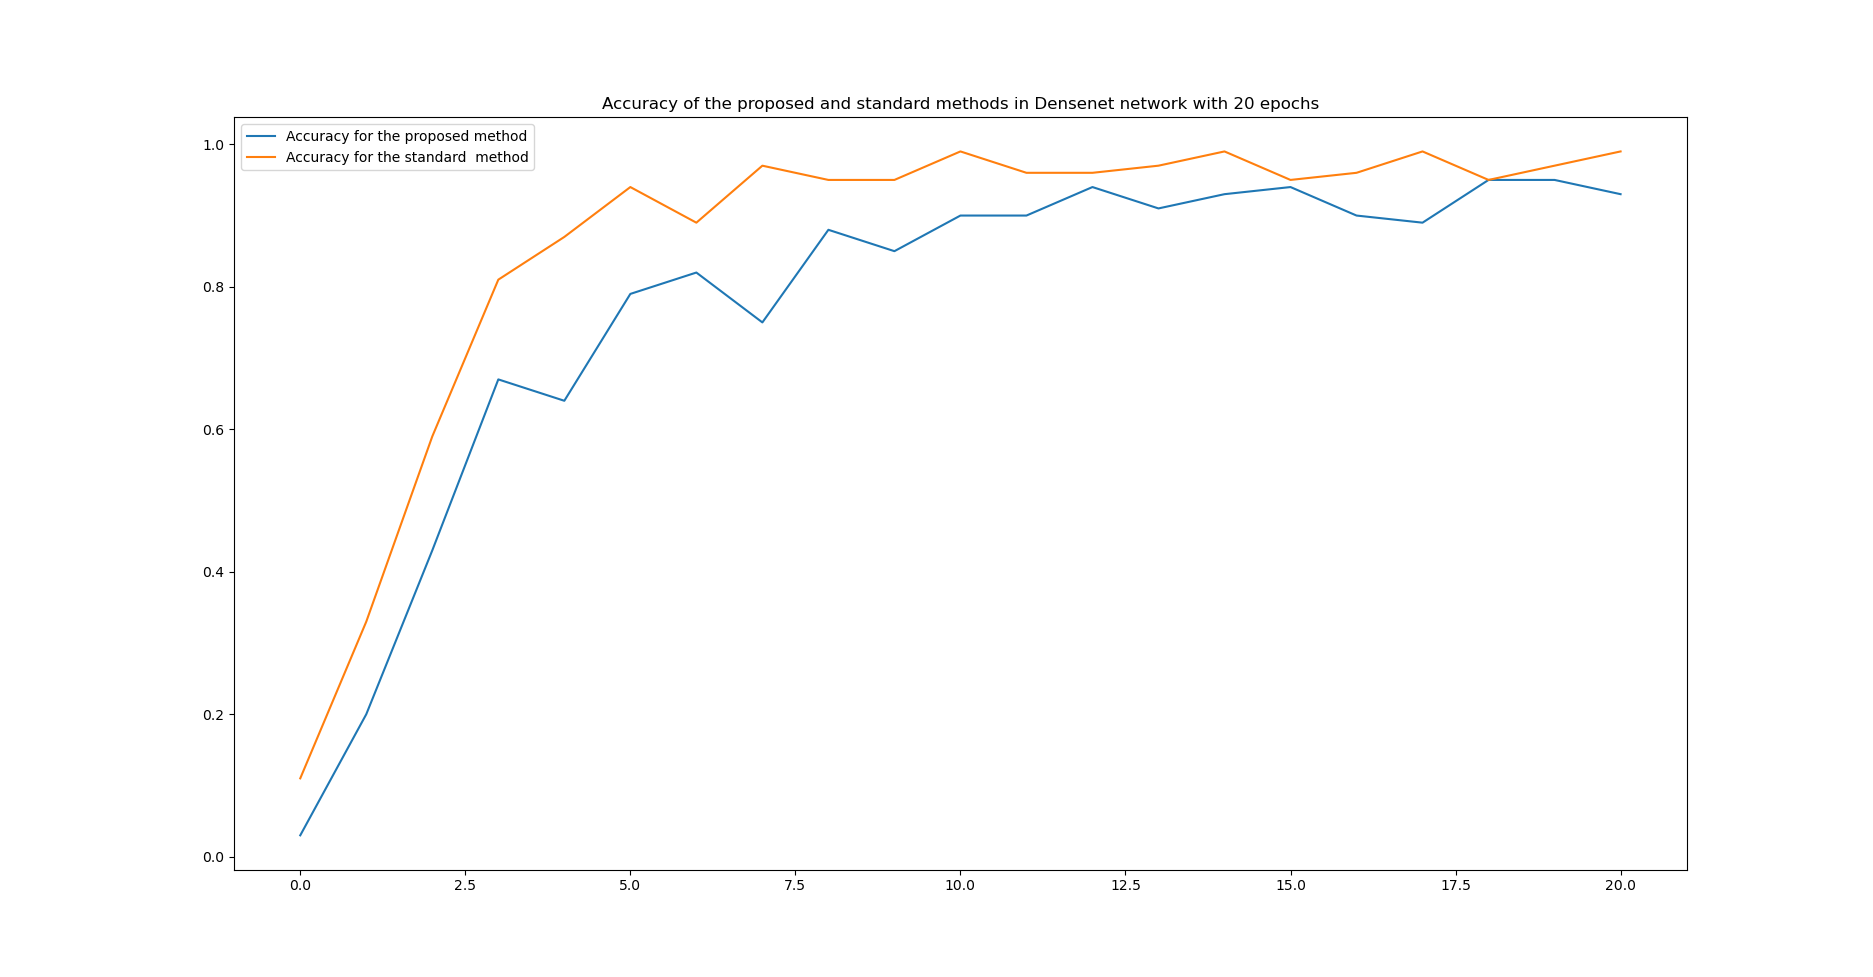
\includegraphics[height=8cm]{Densenet_accuracy_mnist.png}
	\end{center}
	\label{mnistacc}
	\caption{Having the Densenet network trained in 20 epochs, with MNIST dataset with comparable accuracy.
}
\end{figure}



\paragraph*{}
In the process of the whole experiment, we did not use the rank hyperparameter R more than one, and the activation function for all the experiments was ReLU. For the experiments of Densenet network \cite{dense} with the MNIST dataset containing 60000 of 28 by 28-pixel images where the proportion of train to test was 80 to 20, we only used convolutional kernel with three and stride of 1 had only four filters in each convolutional layer. The experiments 
IST via Densenet network are shown in diagrams \ref{mnistacc} and \ref{mnistloss}. For all the experiments alongside bias vectors. Also, we utilized SGD to optimized the networks. On the other hand, All we did to the standard Resnets network was calling the proposed convolution and rerunning the network to compare with the leading network and table
\ref{t1}
were resulted while calling the program with it is default parameters except for the maximum train steps and channels order set to channels-last attribute. We experimented with all the networks trained from scratch, and the trainable variables were initialized with random values.


\begin{figure}[h!]
	\begin{center}
		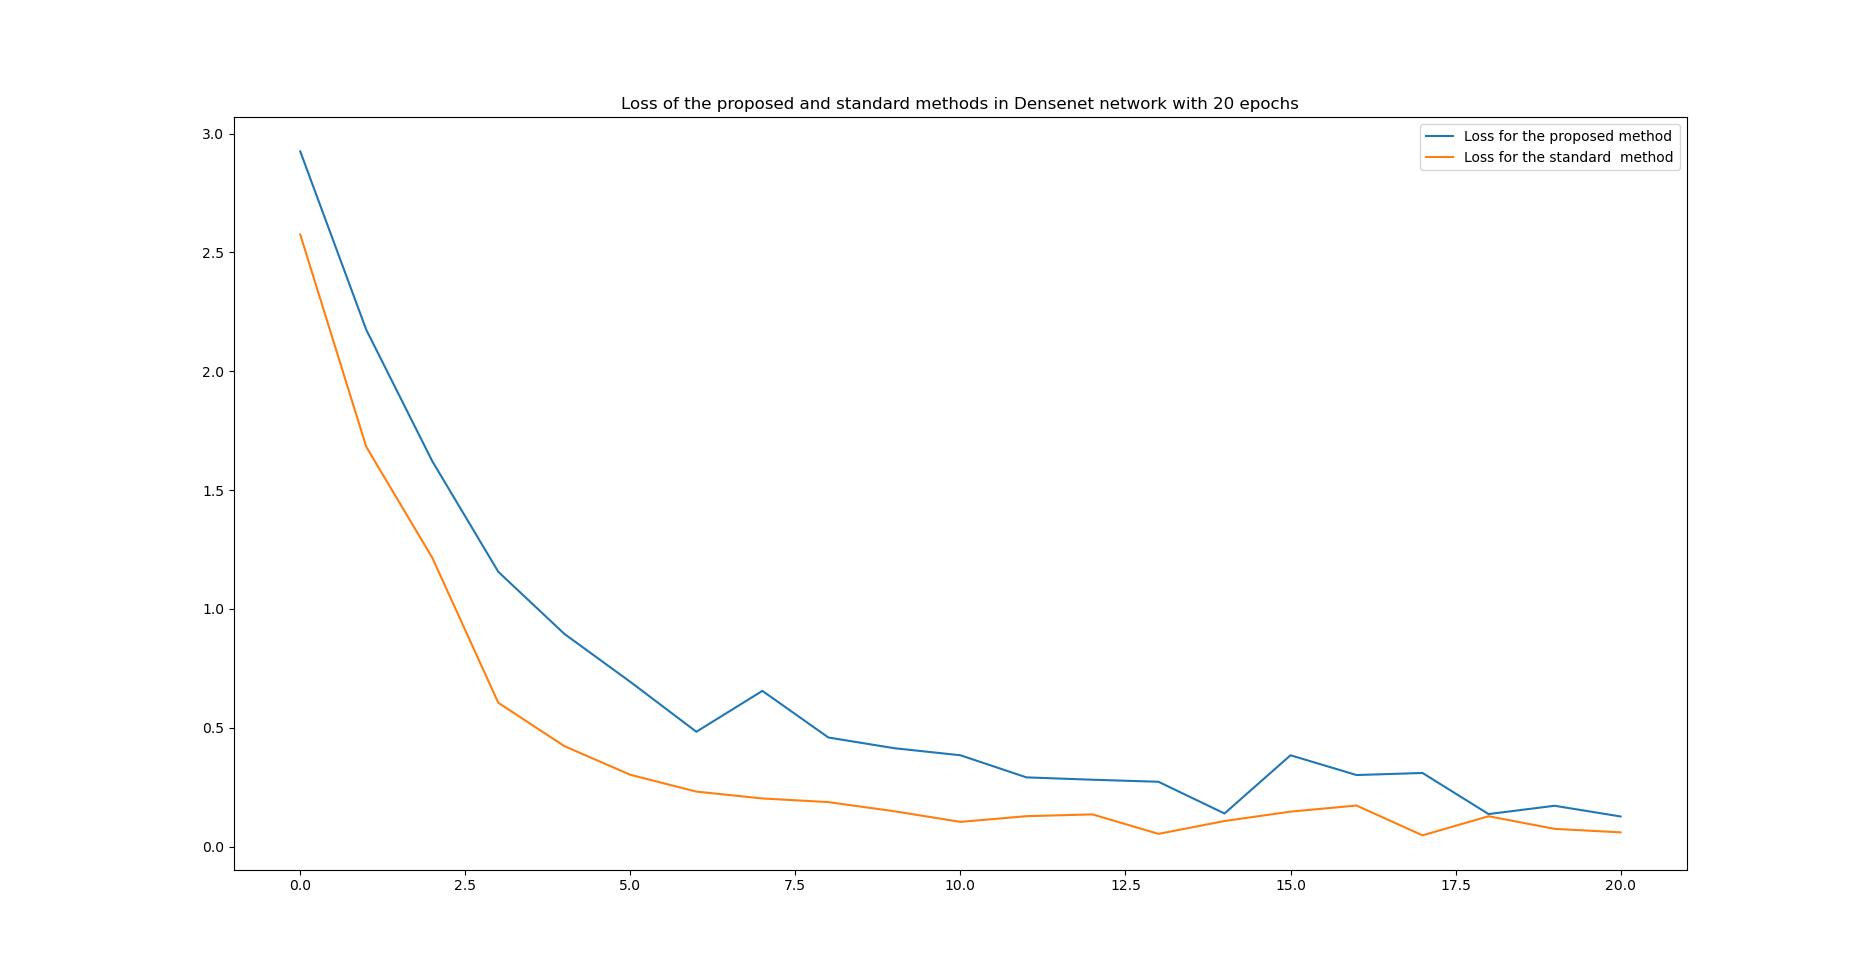
\includegraphics[height=8cm]{densenet_mnist_loss.png}
	\end{center}
	\label{mnistloss}
	\caption{Having the Densenet network trained in 20 epochs, with MNIST dataset we can reach promising loss.
	}
\end{figure}




\begin{table}
	\begin{center}
		\caption{
			The results of experiments with the standard Resnets
			26 in 20000 iterations and 
			Resnets
			56
			with proposed convolution with 40000 and 45000 iterations with Cifar-10 data, respectively. Also in the last row, sum of the calculations during the whole training phase has been reported.
		}
		\label{t1}
		\begin{tabular}{c|c|c|c|c|c|c}
			%\rowcolor{green}
			Row &  
			\thead {
				20000 it\\
				Standard
				\\
				ResNets-26 \\Accuracy}
			&
			\thead {
				20000 it\\
				Standard
				\\
				ResNets-26 \\Loss}
			&
			\thead {
				40000 it\\
				Proposed
				\\
				ResNets-56 \\Accuracy}
			&
			\thead {
				40000 it\\
				Proposed
				\\
				ResNets-56 \\Loss}
			&
			\thead {
				45000 it\\
				Proposed
				\\
				ResNets-56 \\
				Accuracy 	}
			&
			\thead {
				45000 it\\Proposed
				\\
				ResNets-56  \\Loss}
			
			\\&&&&&&	\\
			\hline &&&&&&\\
			1 & 76.99 &    0.99 & 71.87 &  0.93  &  78.12  &  0.73	\\&&&&&&	\\
			2 & 74.75 &    0.98  & 75.00 &   0.87&  78.90  & 0.70	\\&&&&&&	\\
			3 & 70.84 &    1.21 & 69.53 &  0.90 &  76.56  & 0.93	\\&&&&&&	\\
			4 & 75.67 &    1.01  & 73.43 &  0.80 &  78.90  & 0.70	\\&&&&&&	\\
			5 & 75.60 &    1.01  & 78.90 &  0.84 &  78.90  &  0.74	\\&&&&&&	\\
			6 & 82.35 &    0.81  & 76.56 & 0.85  &  78.90  & 0.80	\\&&&&&&	\\
			7 & 86.50 &    0.83  & 80.46 & 0.79  &  78.12  &  0.71	\\&&&&&&	\\
			8 & 82.06 &    0.82  & 73.43 & 0.88  &  76.56  &  0.80	\\&&&&&&	\\
			9 & 71.18 &    1.19  & 75.25 & 0.84  &  78.12  & 0.76	\\&&&&&&	\\
			10 & 74.98 &    1.07 & 78.12    &  0.77   &  75.00  & 0.85	\\&&&&&&	\\
			\hline 	&&&&&&	\\
			Avg
			& 76.49 & 0.99    & 75.00 & 0.84  & 77.80 & 0.77 \\	&&&&&&	\\
			\hline 		\\
			
			Calculations
			
			&\multicolumn{2}{c}{$1.31864168 \times 10^{12}$ }& \multicolumn{2}{c}{$1.32904 \times 10^9$}&
			\multicolumn{2}{c}{$1.49517 \times 10^9$}
			
			\\
		\end{tabular}
		
	\end{center}
\end{table}



\paragraph*{}
Having these settings,datasets and topologies we performed 10 experiments on both proposed or standard resnets lead to results reported in table 
\ref{t1}
 mentioning the accuracy and loss for each experiment as well as their corresponding average accuracy and loss and finally, the number of floating point calculations has been reported in the last row. Table \ref{t1} mentions that the the Resnets-56 with proposed method can reach Resnets-56 with the standard convolution with 20000 iterations somwhere between 40000 and 45000 iterations. Table 
 \ref{t2}
  shows the number of parameters used in Resnets-26 and Resnets-56 for the standard convolution, the multilinear and the proposed method, respectively. Which means the more the networks expands in terms of depth, the more proposed method shows its advantage over the other two methods. In Resnets-26, the proposed convolution consumes about one third the parameters the standard convolution uses. While in shallower networks it can be slightly less thrifty in parameter usage. The reason is that while we have deeper ResNets networks, we deploy much more parameters and obviously, we expect to use dramatically less parameters in the network. In table 
\ref{t3}
 we have reported the count of floating-point calculations during each iteration for ResNets-26 and ResNets-56 with the standard, multinlinear and the proposed convolution, respectively. It is clear that the multilinear and the proposed method have reduced the number of calculations of each iteration, drastically.





\begin{table} 
	\begin{center}
		\caption{
The number of parameters used in 
			ResNets56
			and 
			ResNets26
			for the standard convolution and 
			MLconv 
			and the proposed method
			.
		}
		\label{t2}
		\begin{tabular}{c|c|c|c|c|c|c}
			%\rowcolor{green}
			\thead{
				Network\\ Version }&  
			\thead {
				Standard\\
				Convolution}
			&
			\thead {
				MLconv}
			&
			\thead {Proposed \\Method}
			
			\\
			\hline 	&&&	\\
ResNets-26 &  367280  &  34800 &  29046\\ &&&\\
			ResNets-56 & 851120 &    46960 & 33226
			
			
		\end{tabular}
		
	\end{center}
\end{table}

\newpage

\begin{table}
	\begin{center}
		\caption{
		The number of calculations in 
		ResNets-56
		and 
		ResNets-26
		for the standard convolution and 
		MLconv 
		and the proposed method
		.
		}
		\label{t3}
		\begin{tabular}{c|c|c|c|c|c|c}
			%\rowcolor{green}
			\thead{
				Network\\ Version }&  
			\thead {
				Standard\\
				Convolution}
			&
			\thead {
				MLconv}
			&
			\thead {Proposed \\Method}
			
			\\
			\hline &&& \\
            ResNets-26 &  65932084  &  26905268 &  26716996\\&&&\\
			ResNets-56 & 137284404 &    44950708 & 44658116
			
			
		\end{tabular}
		
	\end{center}
\end{table}















\section{Conclusions}

\paragraph*{}
This paper proposed a new convolution operation and output feature map generation mechanism, which dramatically reduces parameter consumption and calculations. We can flexibly adjust the rank hyperparameter for each convolution to enhance the training ability; meanwhile, we are free to choose the count of the kernels in each filter batch corresponding to each dimension. The memory consumption is exponentially lower than the standard convolution. It can be used in devices and systems with far less computational and memory ability or even a deeper structure. Also, The accuracy and loss results have been shown in the number of parameters and floating-point calculations and the experiments section.

























\bibliographystyle{unsrt}
%\bibliography{references}  %%% Remove comment to use the external .bib file (using bibtex).
%%% and comment out the ``thebibliography'' section.


%%% Comment out this section when you \bibliography{references} is enabled.
\begin{thebibliography}{1}
	
			\bibitem{anim4}
	 N. Cohen, O. Sharir, and A. Shashua. On the expressive power of deep learning: A tensor analysis. CoRR,
	abs/1509.05009, 2015. 1
	
			\bibitem{anim1}
	A. Anandkumar, R. Ge, D. J. Hsu, S. M. Kakade, and
	M. Telgarsky. Tensor decompositions for learning latent
	variable models. Journal of Machine Learning Research,
	15(1):2773–2832, 2014.
	
			\bibitem{anim10}
	 A. Karatzoglou, X. Amatriain, L. Baltrunas, and N. Oliver.
	Multiverse recommendation: n-dimensional tensor factorization for context-aware collaborative filtering. In Proceedings of the fourth ACM conference on Recommender systems,
	pages 79–86. ACM, 2010. 
	
				\bibitem{hinton}
	LeCun, Yann, Yoshua Bengio, and Geoffrey Hinton. "Deep learning." nature 521, no. 7553 (2015): 436-444.
	
\bibitem{vis1}
[1] R. Girshick, J. Donahue, T. Darrell, and J. Malik, “Rich feature
hierarchies for accurate object detection and semantic segmentation,”
in Proceedings of the IEEE conference on computer vision and pattern
recognition, pp. 580–587, 2014.

\bibitem{vis2}
J. Redmon, S. Divvala, R. Girshick, and A. Farhadi, “You only look
once: Unified, real-time object detection,” in Proceedings of the IEEE
Conference on Computer Vision and Pattern Recognition, pp. 779–788,
2016.

\bibitem{vis3} M. A. Waris, A. Iosifidis, and M. Gabbouj, “Cnn-based edge filtering
for object proposals,” Neurocomputing, 2017.

	
					\bibitem{nlp1}
 G. Hinton, L. Deng, D. Yu, G. E. Dahl, A.-r. Mohamed, N. Jaitly,A. Senior, V. Vanhoucke, P. Nguyen, T. N. Sainath, et al., “Deep neural networks for acoustic modeling in speech recognition: The shared views
	of four research groups,” IEEE Signal Processing Magazine, vol. 29,
	no. 6, pp. 82–97, 2012.
	
					\bibitem{nlp2}
	A. Graves, A.-r. Mohamed, and G. Hinton, “Speech recognition with
	deep recurrent neural networks,” in Acoustics, speech and signal processing (icassp), 2013 ieee international conference on, pp. 6645–6649,
	IEEE, 2013.
	
	
	\bibitem{bio1}
	M. Zabihi, A. B. Rad, S. Kiranyaz, M. Gabbouj, and A. K. Katsaggelos,
	“Heart sound anomaly and quality detection using ensemble of neural
	networks without segmentation,” in Computing in Cardiology Conference (CinC), 2016, pp. 613–616, IEEE, 2016.
	
	\bibitem{bio2}
	X. An, D. Kuang, X. Guo, Y. Zhao, and L. He, “A deep learning method
	for classification of eeg data based on motor imagery,” in International
	Conference on Intelligent Computing, pp. 203–210, Springer, 2014.
	
	\bibitem{fin1}
	A. Tsantekidis, N. Passalis, A. Tefas, J. Kanniainen, M. Gabbouj, and
	A. Iosifidis, “Using deep learning to detect price change indications
	in financial markets,” in European Signal Processing Conference (EUSIPCO), Kos, Greece, 2017.

	\bibitem{fin2}
A. Tsantekidis, N. Passalis, A. Tefas, J. Kanniainen, M. Gabbouj, and
	A. Iosifidis, “Forecasting stock prices from the limit order book using
	convolutional neural networks,” in Business Informatics (CBI), 2017
	IEEE 19th Conference on, vol. 1, pp. 7–12, IEEE, 2017.

	
	
	
			\bibitem{anim17}
	H. Sedghi and A. Anandkumar. Training input-output recurrent neural networks through spectral methods. CoRR,
	abs/1603.00954, 2016.
	
			\bibitem{anim9}
	M. Janzamin, H. Sedghi, and A. Anandkumar. Generalization bounds for neural networks through tensor factorization.
	CoRR, abs/1506.08473, 2015.
	
			\bibitem{anim15}
	 V. Lebedev, Y. Ganin, M. Rakhuba, I. V. Oseledets, and
	V. S. Lempitsky. Speeding-up convolutional neural networks
	using fine-tuned cp-decomposition. CoRR, abs/1412.6553,
	2014. 
	
		\bibitem{anim20}
	 Y. Yang and T. M. Hospedales. Deep multi-task representation learning: A tensor factorisation approach. CoRR,
	abs/1605.06391, 2016. 
	
			\bibitem{anim3}
	Y. Chen, X. Jin, B. Kang, J. Feng, and S. Yan. Sharing residual units through collective tensor factorization in deep neural networks. 2017
	
	
	
				\bibitem{resnets}
	He, Kaiming, Xiangyu Zhang, Shaoqing Ren, and Jian Sun. "Deep residual learning for image recognition." In Proceedings of the IEEE conference on computer vision and pattern recognition, pp. 770-778. 2016.
	
	
					\bibitem{mobilenets}
	Howard, Andrew G., Menglong Zhu, Bo Chen, Dmitry Kalenichenko, Weijun Wang, Tobias Weyand, Marco Andreetto, and Hartwig Adam. "Mobilenets: Efficient convolutional neural networks for mobile vision applications." arXiv preprint arXiv:1704.04861 (2017).
	
						\bibitem{alexnet}
	Krizhevsky, Alex, Ilya Sutskever, and Geoffrey E. Hinton. "Imagenet classification with deep convolutional neural networks." Advances in neural information processing systems 25 (2012): 1097-1105.
	
		\bibitem{vgg}
	Simonyan, Karen, and Andrew Zisserman. "Very deep convolutional networks for large-scale image recognition." arXiv preprint arXiv:1409.1556 (2014).
	
	\bibitem{kolda}
	Kolda, Tamara G., and Brett W. Bader. "Tensor decompositions and applications." SIAM review 51, no. 3 (2009): 455-500.

	\bibitem{depthwise}
Chollet, François. "Xception: Deep learning with depthwise separable convolutions." In Proceedings of the IEEE conference on computer vision and pattern recognition, pp. 1251-1258. 2017.

	\bibitem{gpu}
		Lym, Sangkug, Donghyuk Lee, Mike O'Connor, Niladrish Chatterjee, and Mattan Erez. "DeLTA: GPU Performance Model for Deep Learning Applications with In-Depth Memory System Traffic Analysis." In 2019 IEEE International Symposium on Performance Analysis of Systems and Software (ISPASS), pp. 293-303. IEEE, 2019.
		
		\bibitem{danish}
	Tran, Dat Thanh, Alexandros Iosifidis, and Moncef Gabbouj. "Improving efficiency in convolutional neural networks with multilinear filters." Neural Networks 105 (2018): 328-339.
	
	\bibitem{rezghi}
Rezghi, Mansoor, and Lars Elden. "Diagonalization of tensors with circulant structure." Linear Algebra and its Applications 435, no. 3 (2011): 422-447.

	\bibitem{hashteq}
W. Chen, J. T. Wilson, S. Tyree, K. Q. Weinberger, Y. Chen, Compressing neural networks with the hashing trick, in:
Proceedings of the International Conference on Machine Learning (ICML), 2015, pp. 2285–2294.


	\bibitem{prun}
L. Y. Pratt, Comparing biases for minimal network construction with back-propagation, in: Proceedings of the Advances
in Neural Information Processing Systems (NIPS), 1988, pp. 177–185

	\bibitem{redundancy}
Xie, Guotian. "Redundancy-Aware Pruning of Convolutional Neural Networks." Neural Computation 32, no. 12 (2020): 2532-2556.

	\bibitem{fine}
J. Lin, O. Morere, V. Chandrasekhar, A. Veillard, H. Goh, Deephash: Getting regularization, depth and fine-tuning
right, in: Proceedings of the International Conference on Multimedia Retrieval (ICMR), 2017, pp. 133–141.

\bibitem{convop1}
C. Tai, T. Xiao, Y. Zhang, X. Wang, and E. Weinan, “Convolutional neural networks with low-rank regularization,”

	\bibitem{convop2}
J. Ngiam, Z. Chen, D. Chia, P. W. Koh, Q. V. Le, A. Y. Ng, Tiled convolutional neural networks, in: Proceedings of the
Advances in Neural Information Processing Systems (NIPS), 2010, pp. 1279–1287.

	\bibitem{convop3}
M. D. Zeiler, G. W. Taylor, R. Fergus, Adaptive deconvolutional networks for mid and high level feature learning, in:
Proceedings of the International Conference on Computer Vision (ICCV), 2011, pp. 2018–2025.

	\bibitem{convop4}
M. D. Zeiler, D. Krishnan, G. W. Taylor, R. Fergus, Deconvolutional networks, in: Proceedings of the IEEE Conference
on Computer Vision and Pattern Recognition (CVPR), 2010, pp. 2528–2535.

		\bibitem{convop5}
 F. Yu, V. Koltun, Multi-scale context aggregation by dilated convolutions, in: Proceedings of the International Conference
on Learning Representations (ICLR), 2016.
\bibitem{tenmatvec}
Novikov, Alexander, Dmitrii Podoprikhin, Anton Osokin, and Dmitry P. Vetrov. "Tensorizing neural networks." Advances in neural information processing systems 28 (2015): 442-450.

\bibitem{trl}
Kossaifi, Jean, Zachary C. Lipton, Arinbjörn Kolbeinsson, Aran Khanna, Tommaso Furlanello, and Anima Anandkumar. "Tensor regression networks." Journal of Machine Learning Research 21 (2020): 1-21.

\bibitem{dense}
Huang, Gao, Zhuang Liu, Laurens van der Maaten, and Kilian Q. Weinberger. "Densely connected convolutional networks. arXiv 2016." arXiv preprint arXiv:1608.06993 1608 (2018).

\end{thebibliography}


\end{document}
